\documentclass[twoside,onecolumn,11pt,a4paper]{book}
\usepackage{anuthesis}
\usepackage{fancyhdr}
\usepackage{graphicx}

  \renewcommand{\bottomfraction}{0.7}  

\begin{document}

\pagenumbering{roman}  % first use Roman numerals for page numbers

\begin{titlepage}
\title{\textbf{A Simple Example of a Latex Thesis}\\[2cm]}
 \author{\textbf{Mickey M. Mouse}\\[6cm]
 \textbf{A thesis submitted for the degree of}\\
 \textbf{Bachelor of Science with Honours in Physics of} \\
 \textbf{The Australian National University}\\[1cm]}
 \date{\textbf{October, 2004}}
\maketitle
 \end{titlepage}
 
 \sloppy
 
\chapter*{Declaration}
\addcontentsline{toc}{chapter}{Declaration}

This thesis is an account of research undertaken between February 2004 and 
October 2004 at The Department of Physics, Faculty of Science, 
The Australian National University, Canberra, Australia.

Except where acknowledged in the customary manner, the material 
presented in this thesis is, to the best of my knowledge, original and 
has not been submitted in whole or part for a degree in any 
university.

\vspace{20mm}  % vertical space

\hspace{80mm}\rule{40mm}{.15mm}\par   % horizontal space, line, start new line
\hspace{80mm} Mickey M. Mouse\par
\hspace{80mm} October, 2004

% include statements effectively insert the contents of the named file.
% They are not necessary, but are useful for organising your work.
% They always start a  new page.

\chapter*{Acknowledgements}
\addcontentsline{toc}{chapter}{Acknowledgements}

I would like to thank my lucky stars, and the cat, for not eating me.
  % include the contents of the file thanks.tex

\chapter*{Abstract}  % the * means don't put a number in the title
\addcontentsline{toc}{chapter}{Abstract} % but add it to the table of contents

This thesis tells a great story about what I achieved in my research project. The abstract is short, but informative. it makes clear the general area in which I worked, and what I achieved.

  % include the file abstract.tex

\tableofcontents
\listoffigures % makes a list of figures
%\listoftables  % uncomment this if you have tables

\pagenumbering{arabic} % switch to Arabic numerals for page numbers
\setcounter{page}{1}  % set page number to 1

\pagenumbering{arabic} % switch to Arabic numerals for page numbers
\setcounter{page}{1}  % set page number to 1

\chapter{Figures and References}

This chapter gives examples of how to reference the literature, and how to include a figure. To use Latex effectively you either need someone you can ask questions of, or a good book. The book I find most useful is Math into Latex \cite{math into latex}.

You will want reference papers \cite{unruh} and books \cite{pethick}.

Here's an example of including a figure. Figures need to have size information in them. The only ones I know how to make work are encapsulated postscript files, or eps files. If your figures are not in eps form you may need to find a graphics program which can convert formats.
% The percent symbol indicates a comment which is not read by Latex. 
%They are useful because a blank line, means a new paragraph.
\begin{figure}
  \begin{center}  % center environment centers the graphic on the page
    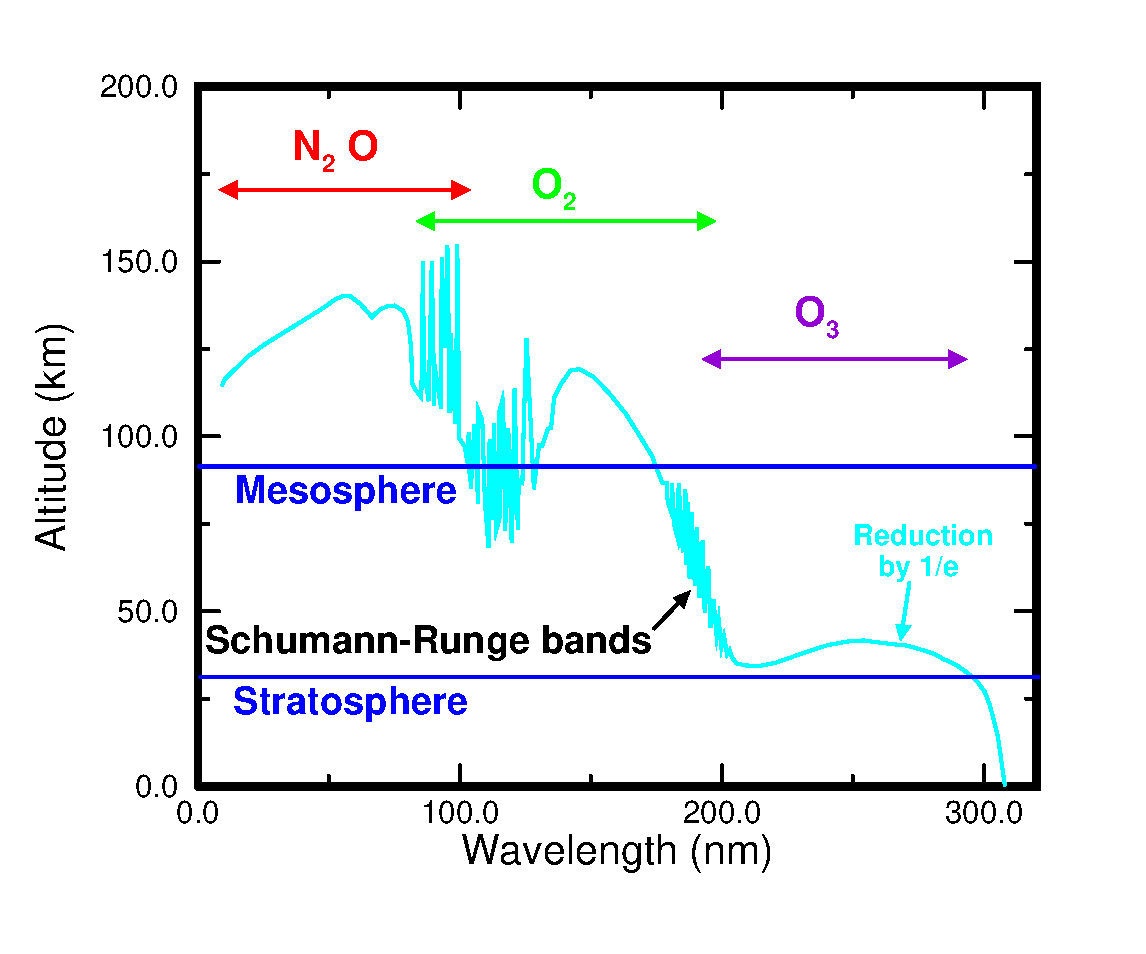
\includegraphics[width=10cm]{fig1.eps}
  \end{center}
\caption{This is an example of how to include an eps (encapsulated postscript) figure. Maths is OK in the caption $\epsilon^2 =\Delta$. }
\label{some text as a figure label}
\end{figure}
%
Notice how I can refer to the figure, Fig.~\ref{some text as a figure label}. 
  % include the file chapter1.tex

\chapter{How to do Maths}

This chapter gives some examples of including maths into your thesis.

An example of a differential equation:
%
\begin{equation} 
\frac{\partial^2 \psi}{\partial t^2} -2i \frac{m v_\theta}{r} \frac{\partial \psi}{\partial t} -
\frac{1}{r} \frac{\partial}{\partial r} \left( r c^{2} \frac{\partial \psi}{\partial r} \right) 
+ \frac{m^{2}}{r^2} \left( c^{2} - v_\theta^{2} \right)  \psi  
= 0 \; .
\label{wave equation}
\end{equation}
%
Equations can also be inline $\phi (t, r, \theta, z) = \psi(t,r) e^{-i m \theta}$, i.e. not displayed separately from the text. I can also refer to equations, Eq.~(\ref{wave equation}).
 % include the file chapter2.tex

% This is an example bibliography file

\begin{thebibliography}{99}  % The 99 becomes 999 if you have more than 99 references

\bibitem{math into latex} ``Math Into Latex'', by George Gr\"{a}tzer, Birkhauser, Boston, 2000.

\bibitem{unruh} Unruh, W.G., Phys. Rev. Lett. 46, 1351 (1981).

\bibitem{pethick} ``Bose-Einstein Condensation in Dilute Gases'', by C.J. Pethick and H. Smith, Cambridge University Press, United Kingdom, 2002.

\end{thebibliography}
  % include the file MyBibliography.tex

\end{document}
